	This interface unifies the management, analysis and reporting stages in one single interface. The most attractive functionalities from this interface is the visualisation of real-time survey responses while interviews are taking place. For that purpose, this interface provides different chart types for each type of question. 

	For instance, Figure \ref{fig:impl:analysisInterface} represents for each interviewee (e.g. y axis), her response to an open-ended question enclosed in one of the six categories (e.g. strong positive, positive, weak positive, weak negative, negative or strong negative) through x axis. This functionality could help to quickly analyse whether or not the responses obtained for an open question match with the survey requirements.

	\begin{figure}[h]
	\centering
	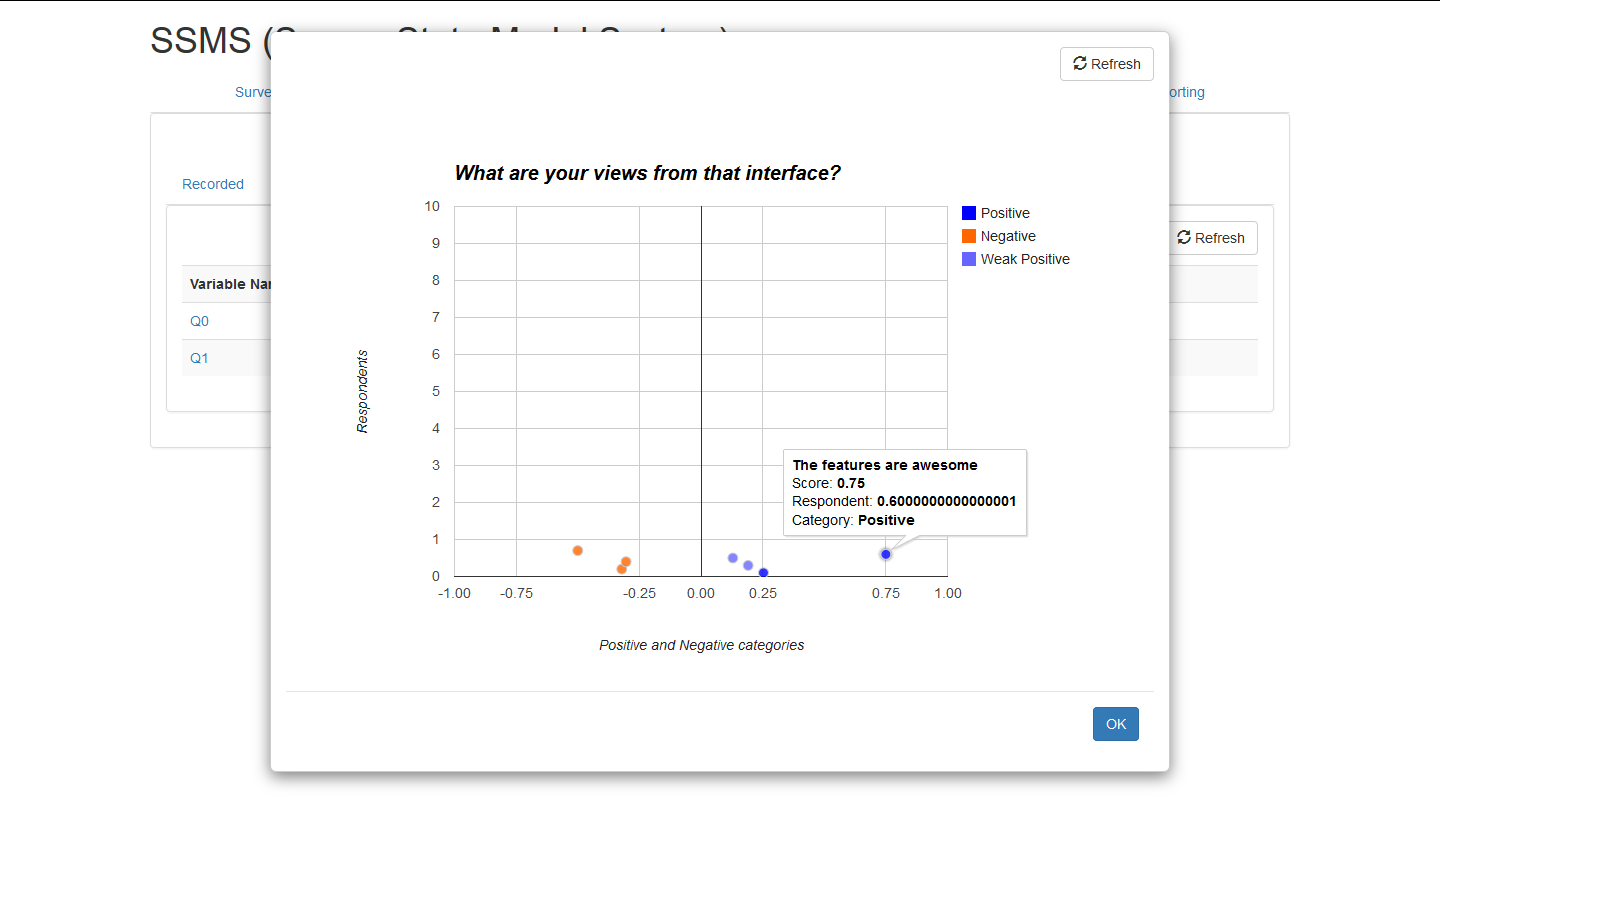
\includegraphics[max size={\textwidth}{\textheight}]{implementation/img/analysis.png}
	\caption{Analysis interface}
	\label{fig:impl:analysisInterface}
	\end{figure}